\section{Eksempel}
Her følger et eksempel på brugen af Mediator pattern. Kildekoden kan ses på github\footnote{\url{https://github.com/BjornNorgaard/I4SWD/tree/master/MediatorPattern}} I eksempelet vil afledte klasser af typen \textit{Participant} kommunikere indbyrdes. Eksempelet er holdt simpelt idet at klasserne via Mediatoren kun kan sende \textit{strings} til hinanden, men selvfølgelig ville dette kunne ændres til hvad end man har brug for.

\begin{lstlisting}
static void Main(string[] args)
{
	Mediator Chatroom = new Mediator();
	
	Participant Dennis = new Borger("Dennis");
	Participant Joachim = new Borger("Joachim");
	
	Chatroom.Register(Dennis);
	Chatroom.Register(Joachim);
	
	Dennis.Send("Joachim", "Herro Jokke!");
	Joachim.Send("Dennis", "Hello Dennis");
}
\end{lstlisting}

Hele klassediagrammet for programmet kan ses på figur~\ref{fig:mediclass} på side~\pageref{fig:mediclass}. En \textit{Participant} har et Mediator medlem og denne bliver sat med \textit{Chatroom.Register(''Parcipant'');} metoden. Hvorved Mediatoren sætte sig selv som netop denne mediator. Implementering ses her:

\begin{lstlisting}
// you can search for complex class with simple key, i.e. string in this case
protected Dictionary<string, IParticipant> Participants;

public virtual void Register(IParticipant participant)
{
	// checking if participant is already in dictionary
	if (Participants.ContainsValue(participant) == false)
		Participants[participant.Name] = participant;
	
	// adding this mediator object to participant when registering
	participant.Mediator = this;
}
\end{lstlisting}

Det er også i Mediatorens \textit{Register} metode at den indeksere det gældende object af typen IParticipant, i dette tilfælde ved \textit{Name} af typen \textit{string}. 

Når en Participant vil sende en besked skal den bare kende modtagerens navn og kalde sin mediators \textit{Send} metode, som det kan ses herunder:

\begin{lstlisting}
public virtual void Send(string to, string message)
{
	// Name being the "return-address"/Senders name
	Mediator.Send(Name, to, message);
}
\end{lstlisting}

Når Mediatoren så skal videreformidle denne besked skal den blot kalde modtagerens \textit{Receive} funktion.

\begin{lstlisting}
public virtual void Send(string from, string to, string message)
{
	// using dict's key as receiver, no need for actual value/object
	IParticipant participant = Participants[to];
	
	if (participant != null)
		participant.Receive(from, message);
}
\end{lstlisting}

Herefter kan modtageren så gøre med besked hvad den nu skal. I dette eksempel vil den blot lave en udskrift:

\begin{lstlisting}
public virtual void Receive(string from, string message)
{
	Console.WriteLine(from + " to " + Name + ": " + message);
}
\end{lstlisting}

Her følger klassediagrammet for implementering af eksemplet:

\begin{figure}[h]
	\centering
	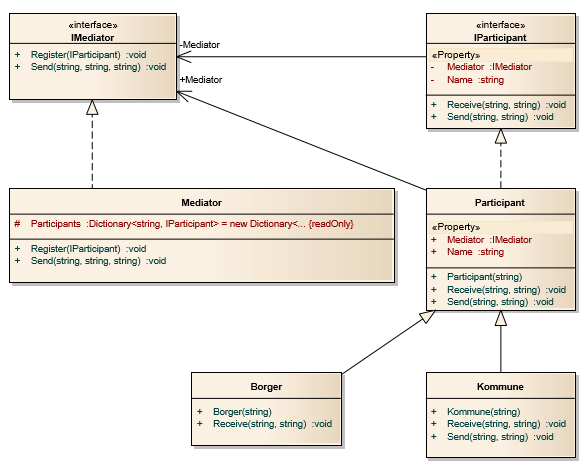
\includegraphics[width=\linewidth]{figs/classdiagram}
	\caption{Klassediagram for vores eksempel på Mediator pattern.}
	\label{fig:mediclass}
\end{figure}